\chapter{Dataset}
In order to train the parameters of the geometric matching CNN model, it is necessary to design the appropriate dataset architecture with suitable training data. The dataset includes two parts. The first part is the images that we use to train the model, this includes both source images and target images. The target image is generated from the source image by an affine transformation. The second part of our training data is the transformation between the source image and target image, the affine transformation, which serve as the label during the training process. We will address the dataset in this chapter.
\section{API}
We use the $google\ map\ static\ api $ to get our high quality aerial images of Prince Edward Island. We select the aerial images by providing the longitude and latitude values to access an image location. The API also has ability to choose the size of an image, also the center of the image. 

\begin{figure}
 \centering
    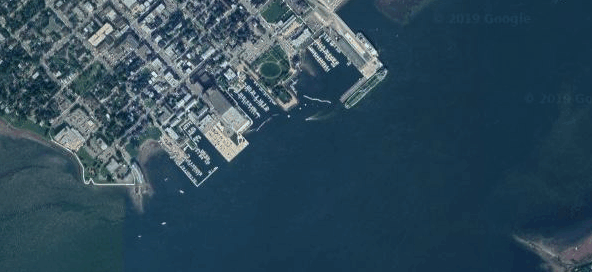
\includegraphics[width=3.0in]{figs/charlottetown}
    \caption{46.2382° N, 63.1311° W, Charlottetown}
\end{figure}


\section{Image}

For training our neural network, an image containing a black bar with unknown data is of no use, we must know what data is supposed to be where the black bar is. In other words we need to know what the aerial photograph should look like if taken from that vantage point. To solve this issue we have come up with the following strategy.\\
  We take a big picture and crop the center square of this big picture. Call this center square the \textit{source image}. Now apply an affine transformation (a rotation or shift or both) to the center square in the big picture. This affine transformation will move the square to some new location and orientation in the big picture. Cropping the big picture using this new square at its new location gives our \textit{target image}. See Figure 3.3. We have that the source image * transformation = target image and there is now no unknown data (no black bars). The source and target images are the inputs to our CNN model. While the transformation matrix serves as the label for supervised training.
\begin{figure}
 \centering
    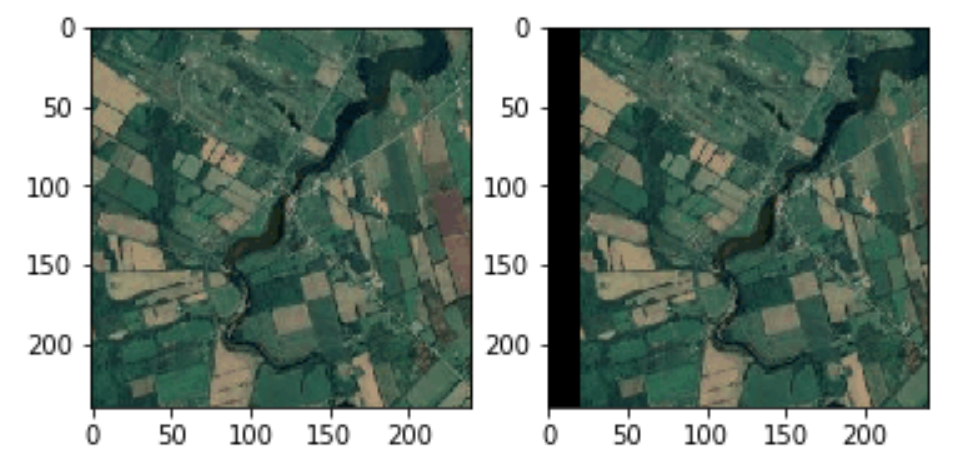
\includegraphics[width=4.0in]{figs/affine_noise}
    \caption{Applying an affine transformation to the image at left, yields the transformed image at right. Notice the black bar on the left side of the transformed image.}
\end{figure}

\section{Training data}
The training dataset includes the source images and the target images. We generated the source images from the API from the previous section, generated the target images by applying transformations to source images.\\
  From each source image, we generate 195 target images by applying a variety of different affine transformations to the source image. Each transformation yields a different target image. We applying the affine transformation that can shift the image first, thus generating the different $tx\ ty$ value in an affine matrix $\begin{pmatrix}
 1 & 0 & tx \\
 0 & 1 & ty
 \end{pmatrix}$, which can shift a image up/down and left/right. For each of the shifted image, we can rotate the images by $ 90,\ 180,\ 270$ degrees, respectively thus generating more target images. We do all of our image manipulations to build the dataset of images using opencv\cite{bradski2000opencv}. Thus for each source image, we can shift the image to obtain a new image, or rotate it, or we can applying both shift and rotation to generate many target images. The architecture of the dataset involve the source image, target image and the  labels. 
 The source images and target images are passed to the CNN model at same time, since we are doing the supervised learning, we also need labels associated with the inputs. The labels are the affine transformation that aligns the source image over top of the target image. If we were generating shift images and rotation images, we will multiple the shift matrix and rotation matrix together. Thus we have a training set containing source images, target images and affine transformations that align a source image with a given target image, this is all the requirements for our supervised machine learning task. We generate 10,000 image pairs including corresponding affine transformation matrices to facilitate our supervised training task. An example of a source and target image are shown in Figure 3.3.

 
\begin{figure}
\centering
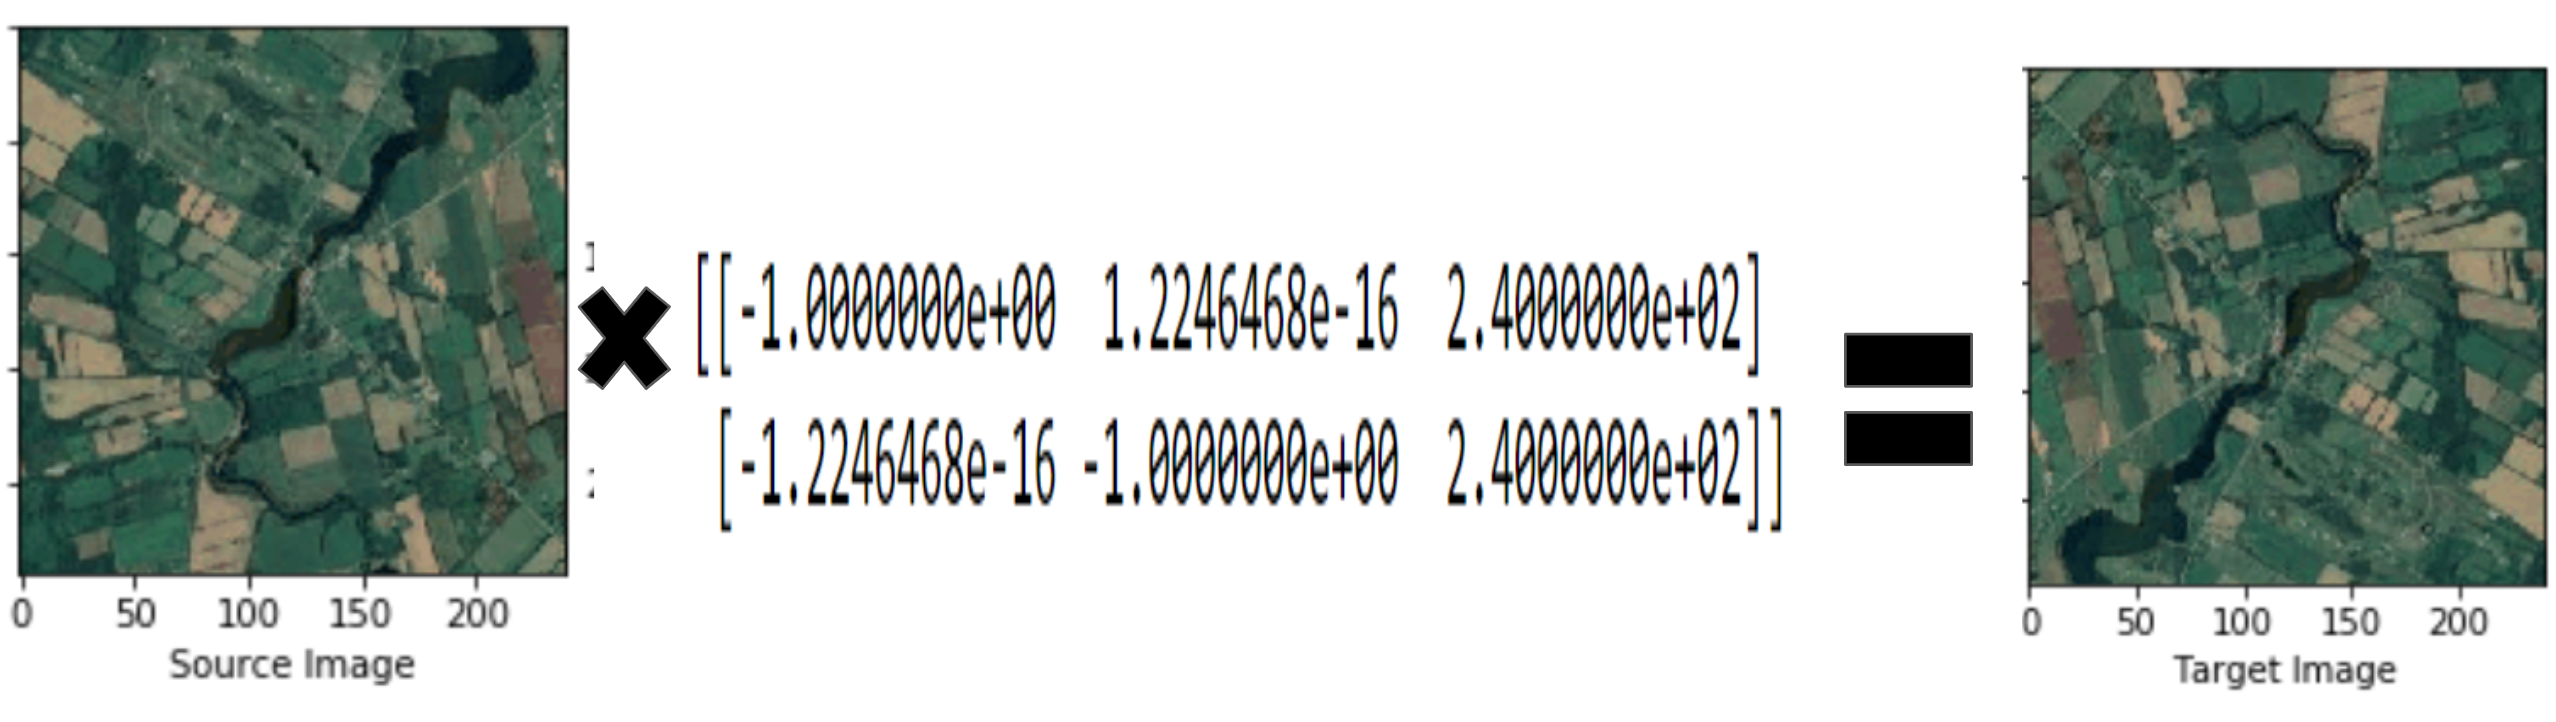
\includegraphics[width = 4.5in]{figs/source_target}
\caption{training image pair}
\end{figure}

\section{CSV File}
In order to access the images and the transformation from the code, we need to be able to store the data in some manner. We choose to store the data in a csv file containing the following information: 
\begin{itemize}
\item path to the source images
\item path to the transform(target) images
\item the affine transformations associated with the source and target images.
\end{itemize}
The affine transformation are labelled as \verb+A00 A01 tx A10 A11 ty+,\\
where A00 gives the entry in the top left corner (0,0) of the affine transformation matrix. The csv files will have at least eight columns includes images paths followed by six columns representing each index in the affine transformation matrix with the order given above.

\section{Format}
In the Feature Extraction part of the CNN model, we are using a pre-trained neural network VGG-16 \cite{simonyan2014very}. The default input images are $ 244 * 244 $, any size changes of the input may change the result of the output. The affine transformations  The VGG16 architecture are shown in Figure 3.4. 
\begin{figure}
 \centering
    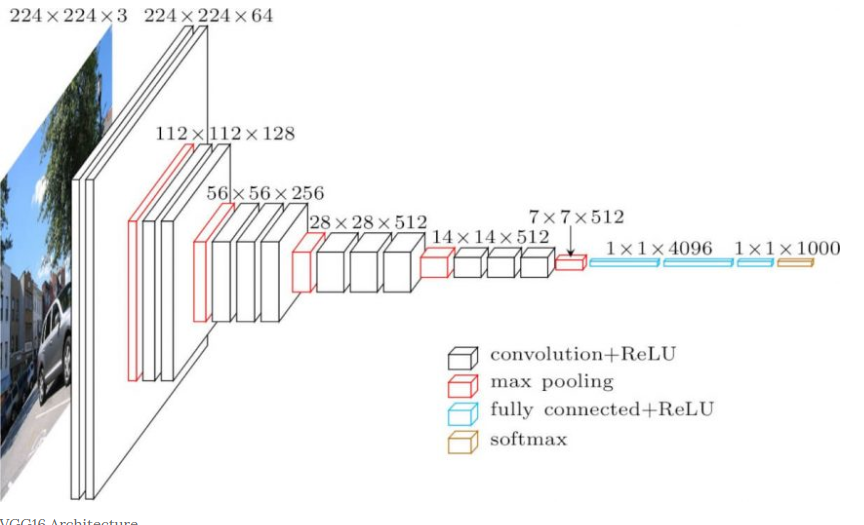
\includegraphics[width=3.0in]{figs/vgg16_architecture}
    \caption{VGG16 Architecture\cite{vgg_arch}}
\end{figure}

  VGG-16 is a convolutional neural network that has already been trained to solve complex image classification tasks. This means it can identify what is in an image (classification). We are not concerned with what is in an image, however as part of VGG-16's training it learns lots of information about images which is then contained within its layers. This information can be thought of as the features that help determine what an image is. We remove the last layers of the VGG-16 network and use the raw data within the layers VGG-16 as our image features. In other words this replaces the traditional task of SIFT to find those interesting portions of an image. These interesting portions of an image are what we call features. This process is outlined in Chapter 2, and is known as transfer learning. We use a pre-trained network and apply its knowledge to help with a different task. In our case we are concerned with finding features within an image (feature extraction), something that VGG-16 is already good at.